%%%%%%%%%%%%%%%%%%%%%%%%%%%%%%%%%%%%%%%%%%%%%%%%%%%%%%%%%%%%%%%%%%%%%%%%%%%%%%%%
%2345678901234567890123456789012345678901234567890123456789012345678901234567890
%        1         2         3         4         5         6         7         8

\documentclass[letterpaper, 10 pt, conference]{ieeeconf}  % Comment this line out if you need a4paper

%\documentclass[a4paper, 10pt, conference]{ieeeconf}      % Use this line for a4 paper

\IEEEoverridecommandlockouts                              % This command is only needed if 
                                                          % you want to use the \thanks command

\overrideIEEEmargins                                      % Needed to meet printer requirements.

% See the \addtolength command later in the file to balance the column lengths
% on the last page of the document

% The following packages can be found on http:\\www.ctan.org
%\usepackage{graphics} % for pdf, bitmapped graphics files
%\usepackage{epsfig} % for postscript graphics files
%\usepackage{mathptmx} % assumes new font selection scheme installed
%\usepackage{times} % assumes new font selection scheme installed
%\usepackage{amsmath} % assumes amsmath package installed
%\usepackage{amssymb}  % assumes amsmath package installed

\usepackage{graphicx}
\usepackage{listings}
\usepackage{array} %don't know why this is needed; get csname error otherwise
\usepackage{tabularx}
\usepackage{float}
\usepackage{caption}
\usepackage{subcaption}

\title{
GreenPlace: A User Driven Marketplace for Perishable Goods\\~\\
Dr. Philip Nico and Dr. Clark Turner, Advisers\\~\\
Computer Science Department\\~\\
College of Engineering\\~\\
June 2015\\
}

\author{Nicolas Higuera}

\begin{document}
\newcommand{\refData}[1]{\textsuperscript{\ref{#1}}}

\onecolumn

\maketitle

\thispagestyle{empty}
\pagestyle{empty}

%%%%%%%%%%%%%%%%%%%%%%%%%%%%%%%%%%%%%%%%%%%%%%%%%%%%%%%%%%%%%%%%%%%%%%%%%%%%%%%%
\begin{abstract}

As the world population grows, food vendors need to be increasingly efficient in the distribution of their products. Products with short shelf-lives need to be distributed as quickly as possible in order to maximize potency. Existing technologies allowing the sale of goods from peer to peer lack key features to optimize usage for perishable goods. GreenPlace provides some of the essential features necessary to distributing perishable goods and managing those orders in an effective manner.

\end{abstract}

\pagebreak
\tableofcontents
\pagebreak

\twocolumn

\section{INTRODUCTION}

Many existing technologies\refData{existing-technologies} allow the peer to peer\refData{peer-to-peer} sale of goods. Though acceptable for most products\refData{product}, these technologies\refData{existing-technologies} are difficult for use by vendors\refData{vendor} of perishable goods\refData{perishable-good}. GreenPlace\refData{greenplace} has a simplified design, is easily accessible, and provides powerful search methods, communication methods, and a product\refData{product} management system all to facilitate peer to peer\refData{peer-to-peer} transactions between vendors\refData{vendor} and consumers\refData{consumer} of products\refData{product} with limited shelf-lives\refData{shelf-life}.

\section{PROBLEMS WITH EXISTING TECHNOLOGIES}

Existing technologies\refData{existing-technologies} like Craigslist function well for the sale of products\refData{product} that do not expire. These technologies\refData{existing-technologies} lack the ability to search products\refData{product} by when the vendor\refData{vendor} is available to conduct a sale. If the fruits on a tree are going to be harvested after a certain date, the farmer would have to add information inside the text post stating when the apples are available. Similarly, users interested in purchasing these apples must individually view each post's content rather than being able to filter by product\refData{product} availability\refData{availability}. Filtering search results based on availability\refData{availability} will simplify the purchasing process of products\refData{product} with limited shelf-lives\refData{shelf-life}.

When searching Craigslist for a product\refData{product}, it can be difficult to filter results based on location. If you wish to search for a product\refData{product} within a 10 mile radius of your current location, you are forced to switch to map view and individually click on each listing to view the title of the link. Craigslist is also separated into seperate subdomains to represent each local area. If searching with a radius extending outside of the local area, the search must be performed under each Craigslist sub-domain. Third party search engines such as www.searchtempest.com exist to solely provide the ability to search all Craigslist for products\refData{product} within a certain distance of your location. Users\refData{user} would benefit through having these map features integrated into a single service.

If a vendor\refData{vendor} wishes to sell a large quantity of products\refData{product} using existing technologies\refData{existing-technologies}, they must either post a single listing representing the sale of all products\refData{product} or multiple listings each representing a fraction of the total quantity available. When the vendor\refData{vendor} is able to sell some of their products\refData{product}, they must manually update the listing to reflect the new quantity available. An ideal marketplace would automatically update the user's\refData{user} listing as products\refData{product} are sold.

\section{TARGET AUDIENCE}

GreenPlace\refData{greenplace} is intended for use by primarily perishable good\refData{perishable-good} producers and consumers: farmers, grocery stores, merchants, and the general public. Producers of local non perishable products could also benefit from using the site as a means of distributing their goods as GreenPlace\refData{greenplace} flexible in design in order to allow the sale of all legal products.

\section{DESIGN AND IMPLEMENTATION}

\subsection{Operating Environment}

GreenPlace\refData{greenplace} is accessible from an HTTP server hosted the cloud using AWS. This allows the software to be accessed by anyone with an internet connection without needing to manually install software locally. Most users\refData{user} currently are aware of how to connect to a website and navigate it with minimal instruction. This operating environment allows GreenPlace\refData{greenplace} to reach a wide audience of users\refData{user} with both internet access and an installed web browser. Node package Forever is used to ensure that the server is restarted in the event of an unexpected crash.

\subsection{Architectural Pattern}

GreenPlace\refData{greenplace} follows a model, view, controller architectural pattern. This allows the model and view components to be reused within the software. As shown in Figure \ref{fig:mvc}, the user\refData{user} interacts with the Jade generated view in order to notify the controller of what actions to perform. The controller uses Express to act upon the AJAX requests sent as a result of user\refData{user} pressing buttons or clicking hyperlinks. Depending on the uploaded data, the controller can decide whether to update the PostgreSQL backend using Sequelize or display a new view to the user\refData{user}.

\section{FEATURES}

\subsection{Tables}

Users\refData{user} have the ability to sort each column by ascending or descending values and filter rows based on provided text on any page containing a table (Figures \ref{fig:searchresults}, \ref{fig:myitems}, \ref{fig:myorders}, \ref{fig:customerorders}, and \ref{fig:receivedmessages}).

\subsection{Authentication}

When a user\refData{user} visits GreenPlace\refData{greenplace} they can choose to log into an existing account\refData{account}, create a new account\refData{account}, or skip authentication and access a limited portion of the site. Creating a new account is as simple as providing a valid email address, username, and password (Figure \ref{fig:authentication}). The provided email address must be validly formatted and neither the username or email address can be in use by an existing user\refData{user}. Authenticating with an existing account\refData{account} is as simple as typing in the username or email and password associated with the user\refData{user}. Once a user\refData{user} has authenticated, it's session is recorded in order to prevent the need for authenticating multiple times during a single usage session\refData{usage-session}.

If authentication is skipped, the user\refData{user} can still access GreenPlace\refData{greenplace} by browsing and searching for posted products\refData{product}. If an unauthenticated user attempts to access any site feature other than browsing, searching, or viewing a product\refData{product}, a prompt for authentication will occur as all other features require an authenticated account\refData{account} for use.

If a user\refData{user} forgets their password, their password can be reset by following the password reset link at the bottom of the authentication page (Figure \ref{fig:authentication}). The user can then input their username or email address and generate a reset url sent to their email address (Figures \ref{fig:resetpassword} and \ref{fig:resetemail}). This url is only valid for thirty minutes, during which the user can set a new password to be associated with their account\refData{account}. If the user attempts to use the reset url outside the reset time window, their password will not be changed.

Note that passwords are hashed, compared, and stored in the database. Once a password has been stored it is never returned to plain text.

\subsection{Searching for Products}

Users\refData{user} can find and view products\refData{product} on GreenPlace\refData{greenplace} by using one of three methods: browsing, searching, or sharing. All of these methods are designed so that first time consumers\refData{consumer} view the benefits of becoming a regular user\refData{user}.

Browsing for a product\refData{product} is done by selecting a location on an embedded map (Figure \ref{fig:browse}). Products\refData{product} are placed on the map as pins as the user\refData{user} pans to new locations or decreases the map scale. When a pin is clicked a box expands showing the product\refData{product} name, description, and vendor\refData{vendor}. The name and vendor are both hyperlinks that open tabs to the product\refData{product} and vendor\refData{vendor} pages respectively.

More specific products\refData{product} can be found through performing a search. Searching is done through initially selecting a single location on a map and specifying a radius around that area where the product\refData{product} must exist (Figure \ref{fig:searchlocation}). After specifying a location and radius the user\refData{user} must provide keywords to look for in the product\refData{product} name and description. Additional criteria which can be provided include time periods in which the vendor\refData{vendor} has marked as available for sale, the minimum quantity of units\refData{unit} available, and a minimum or maximum price for the desired quantity (Figures \ref{fig:searchavailability} and \ref{fig:selectedavailability}). Once the search criteria is filled and submitted, the user\refData{user} is shown all results on a table containing product\refData{product} name, vendor\refData{vendor}, quantity, and price (Figure \ref{fig:searchresults}).

It is worth noting that when searching, the provided availability\refData{availability} is assumed to be provided in the respective timezone in which the product\refData{product} is being sold. That is to say that if the user\refData{user} is located in Los Angeles and searching for products\refData{product} is located in New York, the provided availabilities\refData{availability} are not converted from Pacific Standard Time to Eastern Standard Time, but rather assumed to be provided in Eastern Standard Time. This is to prevent the need for users to manually convert provided availabilities\refData{availability} when searching for products\refData{product} in other time zones. 

\subsection{Purchasing}

Once a consumer\refData{consumer} has found a product\refData{product} they wish to purchase, a button on the product\refData{product} page that when clicked redirects to an order form (Figure \ref{fig:item}). On this form the consumer\refData{consumer} specifies the desired quantity, price, time of sale, and optional message to send to the vendor\refData{vendor}. Once an order has been placed the consumer\refData{consumer} cannot edit the order. If the order was placed by mistake or is no longer valid, the consumer can ``Rescind'' in order to delete the order (Figure \ref{fig:myorders}). 

\subsection{Product Management}

Vendors\refData{vendor} submit their products\refData{product} to GreenPlace\refData{greenplace} by providing the product\refData{product} name, description, image, total quantity, pricing, availability\refData{availability}, and pickup location (Figure \ref{fig:itemnew}). The product\refData{product} description can be formatted using markdown\refData{markdown} to include hyperlinked, bolded, italicized, underlined, and sized text. These fields exist to organize the information for consumers\refData{consumer} browsing GreenPlace\refData{greenplace}. After submission, all product\refData{product} fields can be modified in case a change needs to be made (Figure \ref{fig:itemedit}). Before finalizing changes to an existing or submitting a new product\refData{product}, the vendor\refData{vendor} is shown a page where the post can be previewed. This feature is useful to ensure that the markdown formatted text appears as intended before submission.

If a vendor\refData{vendor} uses other advertising methods to distribute products\refData{product}, they can include a hyperlink to the product\refData{product} page to direct traffic toward their post. The hyperlink allows possible consumers\refData{consumer} to view the product\refData{product} without authentication. The product\refData{product} page includes information regarding the name, description, initial quantity, pricing, availability\refData{availability}, pickup location, and remaining quantity (Figure \ref{fig:item}).

Note that when setting the availability\refData{availability} of a product\refData{product} the times will be set to the respective timezone the product\refData{product} is sold in.

All products\refData{product} listed on the marketplace by the authenticated user\refData{user} can be viewed from they ``My Items'' page (Figure \ref{fig:myitems}). This page provides functionality to view, edit, or delete products\refData{product} currently listed on the marketplace for sale.

Once the product\refData{product} is submitted to the marketplace, the vendor\refData{vendor} is responsible for managing orders placed by other users\refData{user}. The vendor\refData{vendor} can accept or decline the order signifying whether the sale will be completed for on the requested date for the provided quantity and price (Figure \ref{fig:customerorders}). If the order is accepted, the remaining quantity will automatically update relative to the quantity sold in the accepted order. The consumer\refData{consumer} can see the acceptance status\refData{acceptance-status} of their order set by the vendor\refData{vendor}. This establishes a standard means of communication regarding the sale and purchases of products\refData{product} along with the built in messaging system (Figure \ref{fig:receivedmessages}). When changes are made to a product\refData{product}, it's orders are not modified in any way. Accepted orders will remain accepted even if the total quantity is reduced below the number purchased in the accepted order.

Once an order has been placed it's acceptance status\refData{acceptance-status} is set to ``Pending". Orders that are pending can be rescinded by the consumer\refData{consumer} and accepted or declined from the vendor\refData{vendor} only if the order's status is ``Pending". Once a change has been made by the consumer\refData{consumer} or vendor\refData{vendor} the status cannot be changed. Users\refData{user} are encouraged to share more specific information regarding the purchase such as contact information and directions once an order has been placed. Note that an order cannot be placed on a product\refData{product} owned by the same user.

\subsection{Interfacing with Other Users}

Each account\refData{account} has a customizable profile (Figure \ref{fig:profile}). This profile page allows other users\refData{user} to view public information posted by the account\refData{account} owner. The profile page can include a profile picture and text formatted with markdown\refData{markdown}.

Users\refData{user} can message one another for any reason by clicking a button at the bottom of the user's\refData{user} profile page (Figure \ref{fig:profile}). A message must contain both a subject and description (Figures \ref{fig:message}, \ref{fig:composemessage}, \ref{fig:previewmessage}). All users\refData{user} have an inbox where messages can be viewed and a responses can be sent to the user\refData{user} that sent the message (Figure \ref{fig:receivedmessages}).

\section{PROBLEMS ENCOUNTERED}

\subsection{Database Change}
Originally, GreenPlace\refData{greenplace} was constructed using a combination of MongoDB and Mongoose for the model component. These are relatively new technologies that allow data to be stored in documents rather than the commonly used relational tables. It was a pitfall to assume that newer technologies are always better than the old. With MongoDB, aggregation queries were difficult and impractical to write as they require a lot of boilerplate code. An example of this is where MongoDB in it's current state does not allow performing a query to determine the distance from a location and verifying that it's values are within inside of an array in a single query. This requires two queries to perform a single action and then only displaying the results inside of both queries. This query became resource intensive and showed the weaknesses in the application of MongoDB.

In the second quarter, MongoDB and Mongoose were completely replaced by PostgreSQL and Sequelize. By switching to PostgreSQL, aggregation queries became easier to write and less resource intensive.

\section{FUTURE WORK}

\subsection{Subscriptions / Notification System}
Users\refData{user} should be able to receive email notifications when receiving a message, a new order is placed on one of their products, and specific vendors\refData{vendor} post a new product\refData{product} for sale. This would encourage users\refData{user} to return GreenPlace\refData{greenplace} to conduct business. 

\subsection{Comments / Feedback}
As GreenPlace\refData{greenplace} is in the early development process, feedback from users\refData{user} is important in order to determine features and modifications to consider making. A ``Give Feedback'' hyperlink at the bottom of each page allowing users\refData{user} to send messages to my personal GreenPlace\refData{greenplace} account\refData{account} would be sufficient for gathering feedback from users\refData{user}.

\subsection{Flagging Posts}
As with all online services, some users\refData{user} post inappropriate or illegal content. A method should exist to flag these users\refData{user} and products\refData{product} for removal.

\subsection{View Upcoming Transactions}
When a vendor\refData{vendor} has a large number of orders for a product, it would be beneficial to display them on a calendar. This would allow the vendor\refData{vendor} to view their schedule easily without having to navigate through each order. It may also be beneficial to export this data to an existing calendar service such as Google Calendar.

\subsection{Sharing Contact Information}
After a vendor\refData{vendor} accepts an order placed by the consumer\refData{consumer} both users\refData{user} should be able to access private information regarding eachother such as contact information and first and last name. This will allow both users\refData{user} to communicate outside of GreenPlace\refData{greenplace} before completing a transaction.

\subsection{Usage Terms and Privacy Policy}
Links to usage terms and the privacy policy should be visible at the bottom of each page in order to inform the user\refData{user} of how the site should be used legally and what is being done with user\refData{user} provided data.

\section{CONCLUSIONS}
GreenPlace\refData{greenplace} is a peer to peer\refData{peer-to-peer} marketplace designed for the sale of perishable goods\refData{perishable-good}. The software allows users\refData{user} to find products\refData{product} within a radius from a provided location, communicate with other users\refData{user} through an internal messaging service, and manage their product\refData{product} information and orders in a single location. GreenPlace\refData{greenplace} is a digital farmers market with the tools essential to selling perishable goods\refData{perishable-good}.


%%%%%%%%%%%%%%%%%%%%%%%%%%%%%%%%%%%%%%%%%%%%%%%%%%%%%%%%%%%%%%%%%%%%%%%%%%%%%%%%
\clearpage
\onecolumn
\section{APPENDIX}

\subsection{Technologies Used}

\begin{tabularx}{\textwidth}{l|X|X}
  \textbf{Technology} & \textbf{Description} & \textbf{Resource URL} \\
\hline

Dploy.io & Tool for automatically deploying & http://dploy.io/\\
Amazon Web Services & Server hosting GreenPlace & aws.amazon.com/free‎\\
NodeJS & JavaScript library used to run the HTTP server & https://nodejs.org/\\
Forever & Node package used to keep a node process running without interuptions & https://github.com/foreverjs/forever\\
Jade & Node template engine used to render HTML files & http://jade-lang.com/\\
Passport & Node package used for authenticating users and managing usage sessions & http://passportjs.org/\\
MongoDB & Document database completely replaced by PostgreSQL in the final version of the website & https://www.mongodb.org/\\ 
Mongoose & Node package used to communicate to MongoDB. Completely replaced by Sequelize in the final version of the website. & http://mongoosejs.com/\\
PostgreSQL & Relational database used to user information & http://www.postgresql.org/\\
Sequelize & Object relational mapping used for communicating with PostgreSQL database using JavaScript & http://docs.sequelizejs.com\\
Busboy & Node package used to parse multipart form-data POSTed by users & https://www.npmjs.com/package/busboy\\
Body-Parser & Node package used to parse non multipart form-data POSTed by users & https://www.npmjs.com/package/body-parser\\
Underscore & JavaScript utility package & https://www.npmjs.com/package/underscore\\
Lodash & JavaScript utility package & https://www.npmjs.com/package/lodash\\
Crypto-Js & Node package used for hashing user passwords & https://www.npmjs.com/package/crypto-js/\\
Nodemailer & Node package used to send templated emails & https://www.npmjs.com/package/nodemailer/\\
Email-Templates & Node package used to template emails & https://www.npmjs.com/package/email-templates/\\
Moment & Node package used for manipulating JavaScript Date objects & http://momentjs.com/\\
Moment-Timezone & Node package for converting moments from one timezone to another & http://momentjs.com/timezone/\\
Tzwhere & Node package to determine the timezone of gps coordinates & https://www.npmjs.com/package/tzwhere/\\
Marked & Node package used to parse markdown text into HTML & https://www.npmjs.com/package/marked\\
Express & Handle user AJAX requests & https://www.npmjs.com/package/express\\
Express-Session & Node package used to handle usage sessions without reauthenticating with each page load & https://www.npmjs.com/package/express-session\\
Express-Validator & Node package used to validate user input and sanitize uploaded data & https://www.npmjs.com/package/express-validator/\\
PureCSS & CSS library used to style web pages & purecss.io\\
JQuery & JavaScript utility library & https://jquery.com/\\
JQuery DatePicker & JavaScript library allowing the selection of multiple dates on a calendar & http://keith-wood.name/datepick.html\\
Isotope & JavaScript library used to allow sorting of HTML tables &http://isotope.metafizzy.co/\\
Google Maps JavaScript v3 API & JavaScript library used to allow user map interaction & https://developers.google.com-/maps/documentation/javascript/reference\\
\end{tabularx}

\subsection{Data Dictionary}
% automatically number examples throughout document
\newcounter{exno}
\newenvironment{dictionary} {
   \begin{flushleft}
   \begin{tabular*}{\textwidth}{>{\refstepcounter{exno}\theexno.}l r}
}
{
   \end{tabular*}
   \end{flushleft}
}

\begin{dictionary}
   \hline
   \label{greenplace} GreenPlace &SaaS created to facilitate peer to peer sales of perishable goods\\
   \hline
   \label{peer-to-peer} Peer to Peer &Direct sale and purchase of a product from one user to another\\
   \hline
   \label{product} Product &Anything that is produced and inteded for sale to another party\\
   \hline
   \label{vendor} Vendor &A person or company that sells products to another party\\
   \hline
   \label{consumer} Consumer &A person or company that purchases products\\
   \hline
   \label{user} User &A person or company that uses the website [vendor, consumer]\\
   \hline
   \label{perishable-good} Perishable Good &A product which has a fixed lifespan before it is no longer valid\\
   \hline
   \label{shelf-life} Shelf-Life &The amount of time a product can be left unused before it is no longer able to function properly\\
   \hline
   \label{potency} Potency &The effectiveness of a product to perform its intended purpose\\
   \hline
   \label{existing-technologies} Technology &Other marketplaces intended for peer to peer sales: Craigslist, Ebay, Amazon, etc.\\
   \hline
   \label{account} Account &Digital information that represents the user when using GreenPlace\\
   \hline
   \label{usage-session} Usage Session &Period of time from which a user uses GreenPlace\\
   \hline
   \label{unit} Unit &The unit used to quantify a product: litres, kilograms, and each individual product aka unit\\
   \hline
   \label{acceptance-status} Acceptance Status &Whether an order has been rescinded, accepted, declined, or pending approval\\
   \hline
   \label{markdown} Markdown &Language that allows formatting of text\\
   \hline
   \label{saas} SaaS &Software as a service\\
   \hline
   \label{availability} Availability &The time which a sale can be conducted\\
   \hline
\end{dictionary}

\iffalse
\subsection{Example Use Cases}

The table below illustrates some typical users and the reasons they wish to use the GreenPlace\refData{greenplace}.

\begin{tabularx}{\textwidth}{X|X}
  \textbf{Example Use Cases} & \textbf{Description}\\
\hline
Farmer wishes to advertise local produce for sale & Farmer creates a profile and posts item for sale on the marketplace. The item posted can then be found by interested consumers\refData{consumer}\\
Consumer\refData{consumer} is seeking to purchase bananas & Consumer\refData{consumer} browses or searches their local area for bananas based on the desired quantity, availability\refData{availability}, and price.\\
Vendor\refData{vendor} wishes to keep track of product\refData{product} reserved by consumers\refData{consumer} & After a product\refData{product} is posted to GreenPlace\refData{greenplace}, the remaining quantity is automatically updated upon accepting orders placed by consumers\refData{consumer}.\\
User\refData{user} forgets their password to their account & User\refData{user} clicks the ``Reset Password'' hyperlink on the authentication page and follows the instructions. After sending a reset attempt the user\refData{user} opens their email and clicks the hyperlink to reset the password associated with their account\refData{account}

\end{tabularx}
\fi


\subsection{Figures}

\begin{figure}[H]
  \caption{MVC Diagram}
   \label{fig:mvc}
  \centering
    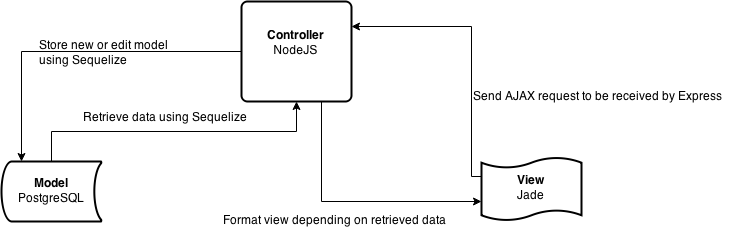
\includegraphics[width=0.5\textwidth]{images/MVC.png}
\end{figure}

\begin{figure}[H]
  \caption{Authentication}
  This is the default screen to an unauthenticated user. From this page the user can login to an existing or create a new account, or browse the marketplace without authenticating.\\
  \label{fig:authentication}
  \centering
    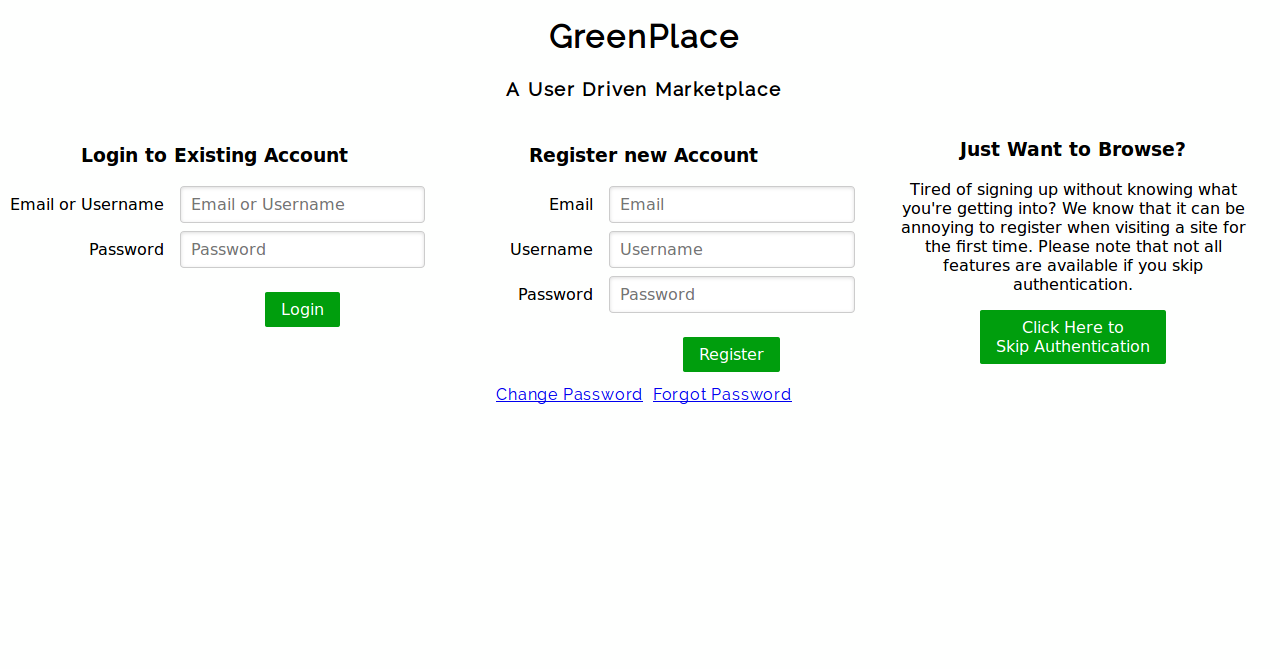
\includegraphics[width=\textwidth]{images/authentication.png}
\end{figure}

\begin{figure}[H]
  \caption{Change Password}
  Accessed by clicking the ``Forgot Password'' hyperlink on Figure \ref{fig:authentication}. Users can change their password by filling in their username or email, old password, and new password.\\
  \label{fig:changepassword}
  \centering
    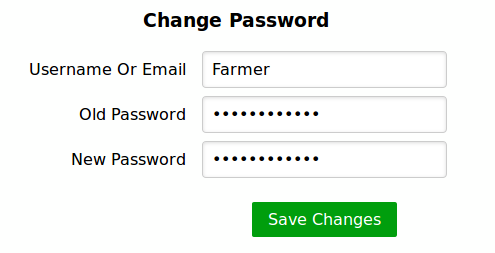
\includegraphics[width=0.5\textwidth]{images/changepassword.png}
\end{figure}

\begin{figure}[H]
  \caption{Reset Password}
  Allows users to reset their password by providing either their username or email address. It is accessed by clicking the ``Reset Password'' hyperlink on Figure \ref{fig:authentication}. After submission, an email is sent to the user's email address depicted by Figure \ref{fig:resetemail}.\\
  \label{fig:resetpassword}
  \centering
    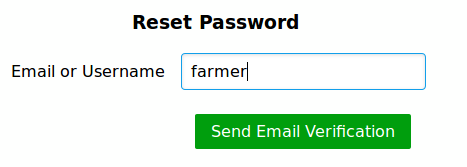
\includegraphics[width=0.5\textwidth]{images/resetpassword.png}
\end{figure}

\begin{figure}[H]
  \caption{Reset Password Email}
  Represents a reset password attempt generated by Figure \ref{fig:resetpassword}. The user can click the reset url in order to change their password.\\
  \label{fig:resetemail}
  \centering
    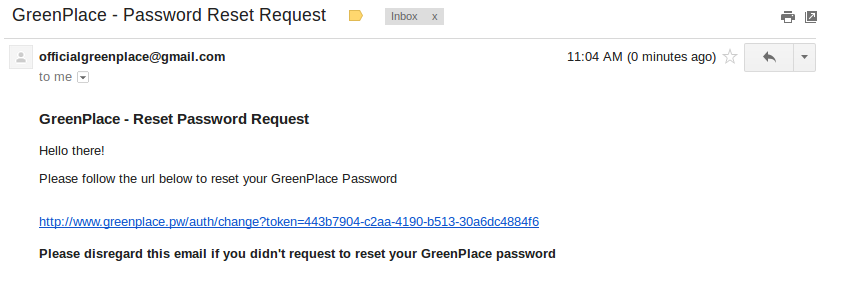
\includegraphics[width=\textwidth]{images/resetemail.png}
\end{figure}

\begin{figure}[H]
  \caption{Browsing the Marketplace}
  Default page for an authenticated user. The user is displayed all items for sale in their area. Users can center the map on their location by pressing the ``Go to Current Location'' button.\\
  \label{fig:browse}
  \centering
    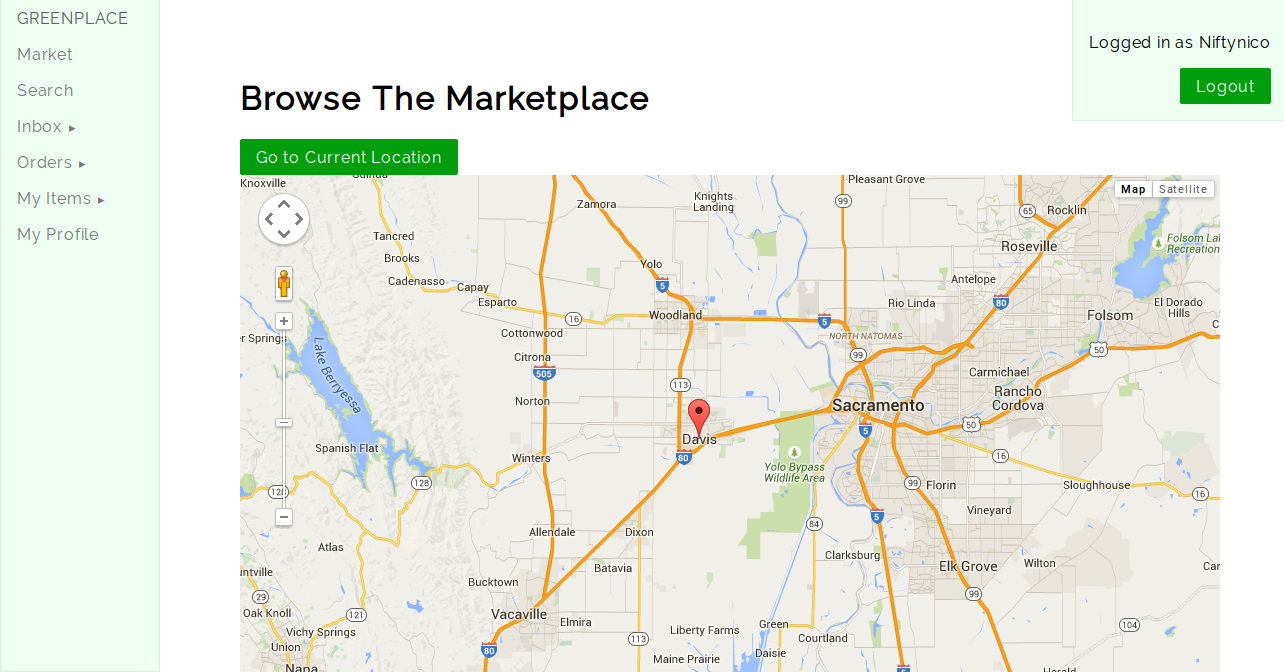
\includegraphics[width=\textwidth]{images/browse.png}
\end{figure}

\begin{figure}[H]
  \caption{Search Location}
  Allows users to set their location and radius to find items in.\\
  \label{fig:searchlocation}
  \centering
    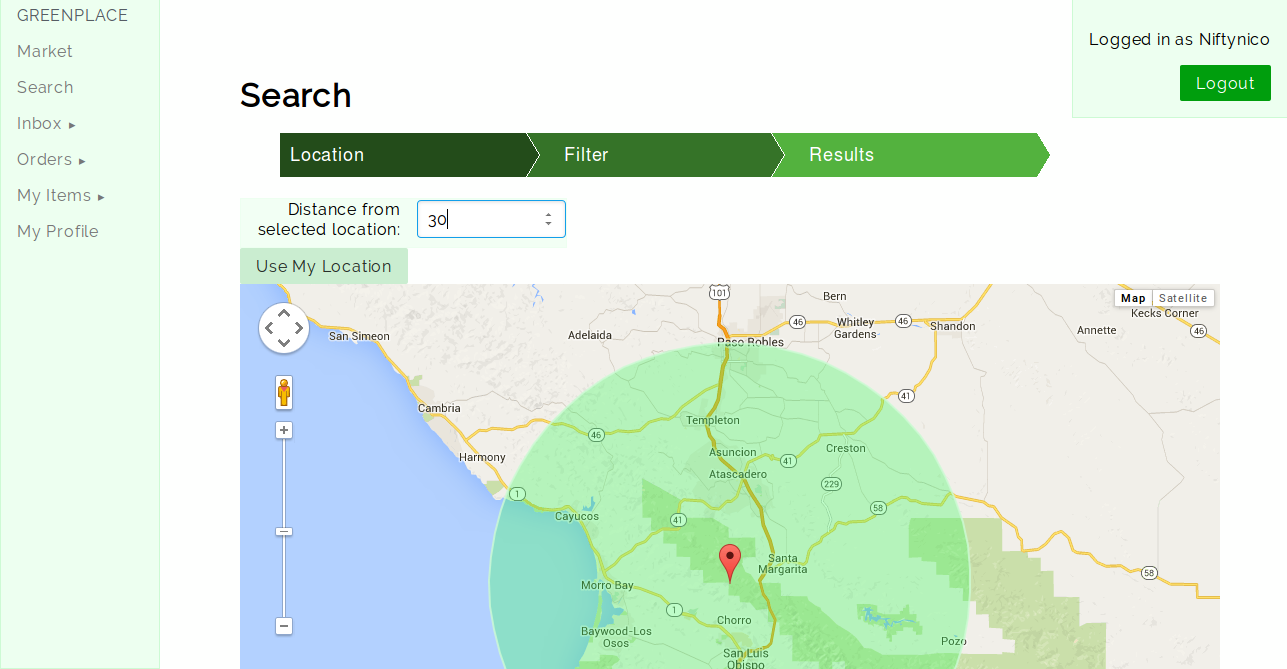
\includegraphics[width=\textwidth]{images/search-location.png}
\end{figure}

\begin{figure}[H]
  \caption{Search - Selecting Availability}
  Select one or more days at once to be added to the search criteria.\\
  \label{fig:searchavailability}
  \centering
    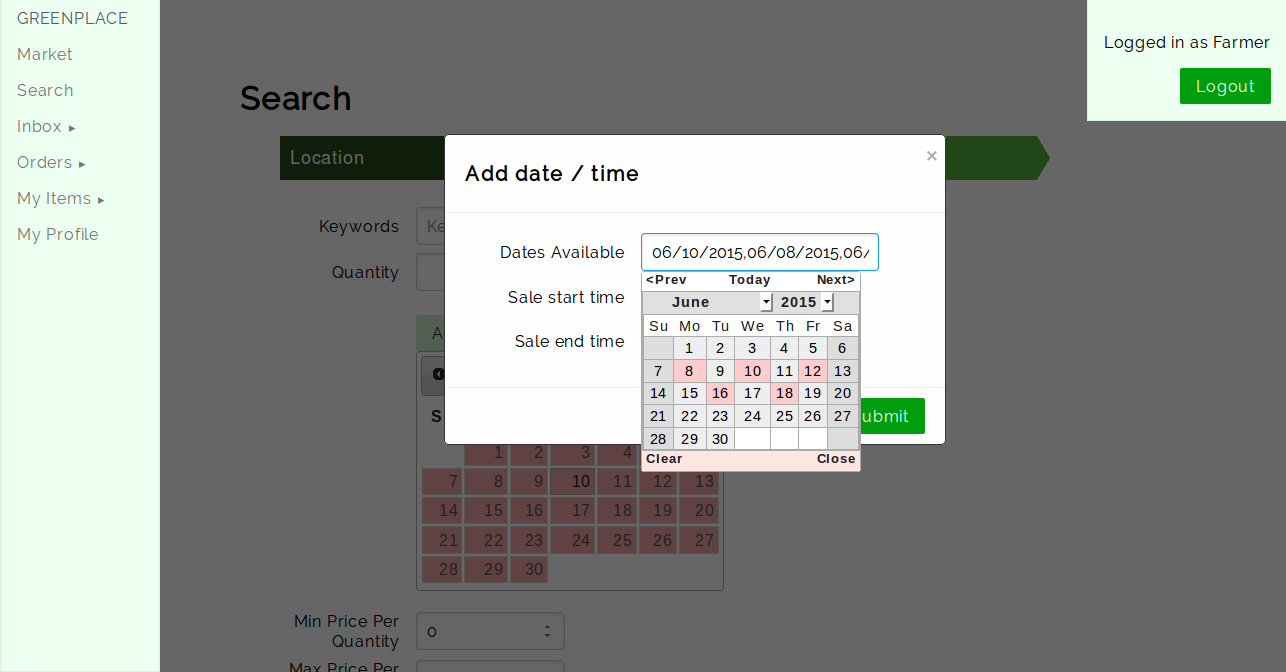
\includegraphics[width=\textwidth]{images/selectmultipledates.png}
\end{figure}

\begin{figure}[H]
  \caption{Search - Selected Availability to Add}
  Set the time period for the selected days to add to the search criteria.\\
  \label{fig:selectedavailability}
  \centering
    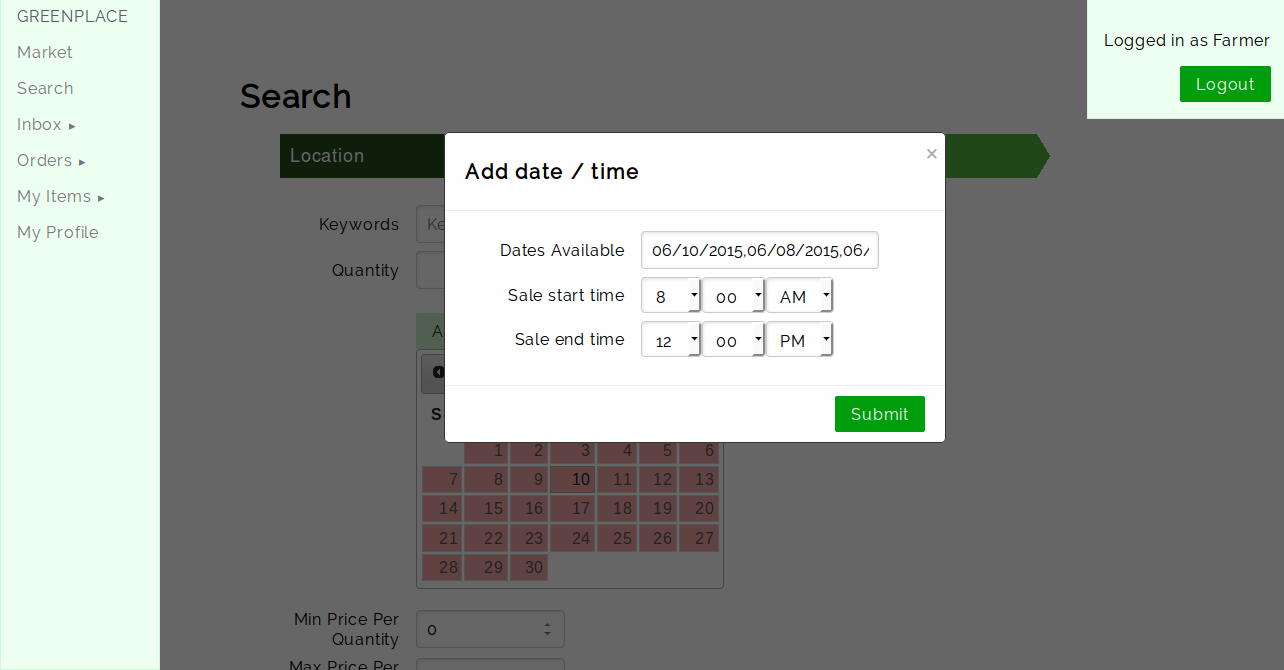
\includegraphics[width=\textwidth]{images/search-availability.png}
\end{figure}

\begin{figure}[H]
  \caption{Search - Results}
  Results when searching for ``Avocado'' near San Luis Obispo.\\
  \label{fig:searchresults}
  \centering
    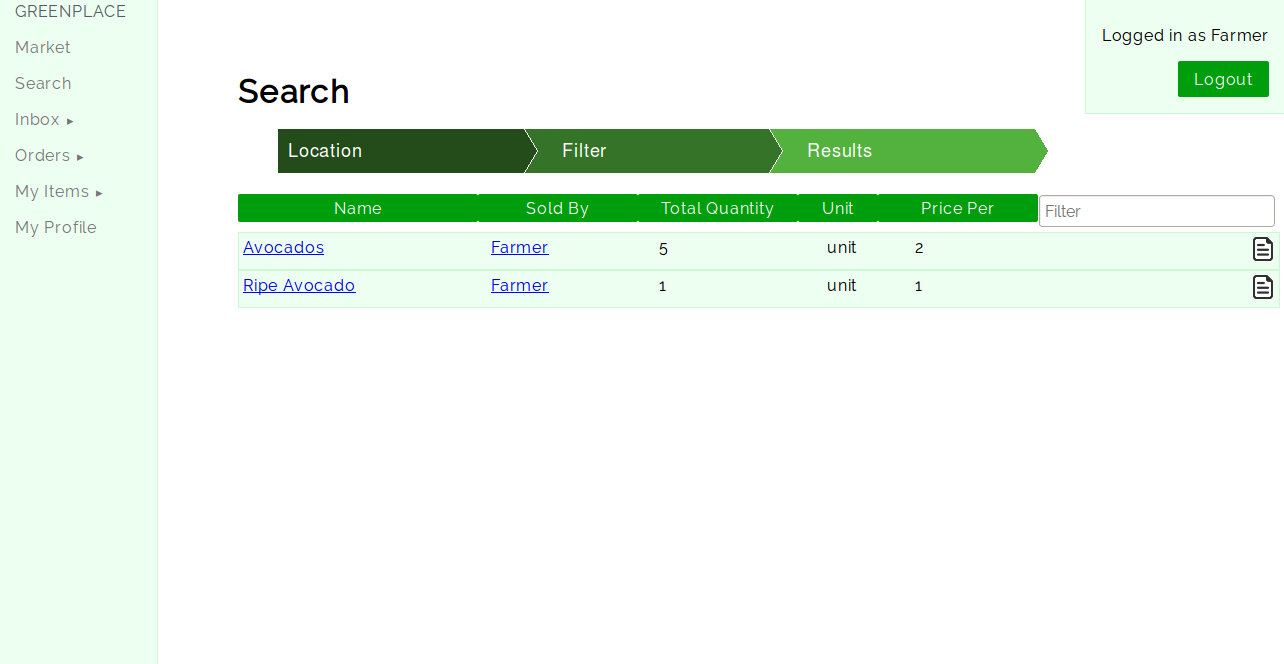
\includegraphics[width=\textwidth]{images/searchresults.png}
\end{figure}

\begin{figure}[H]
  \caption{New Item}
  Template to be filled by the user to represent the product for sale.\\
  \label{fig:itemnew}
  \centering
    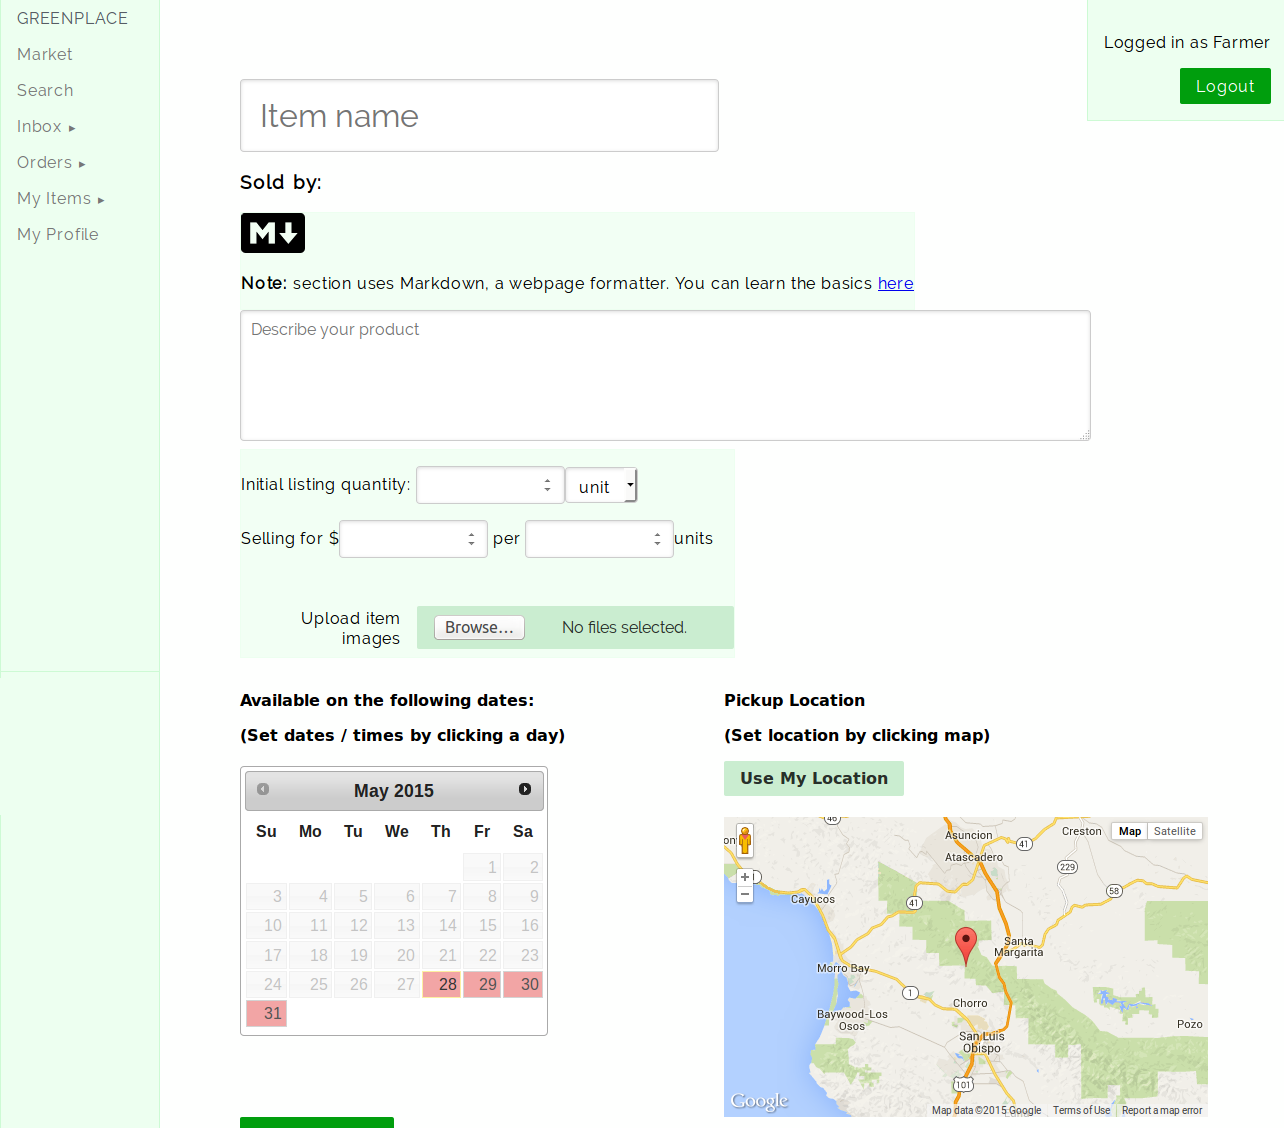
\includegraphics[width=\textwidth]{images/itemnew.png}
\end{figure}

\begin{figure}[H]
  \caption{Item}
  Represents a product for sale.\\
  \label{fig:item}
  \centering
    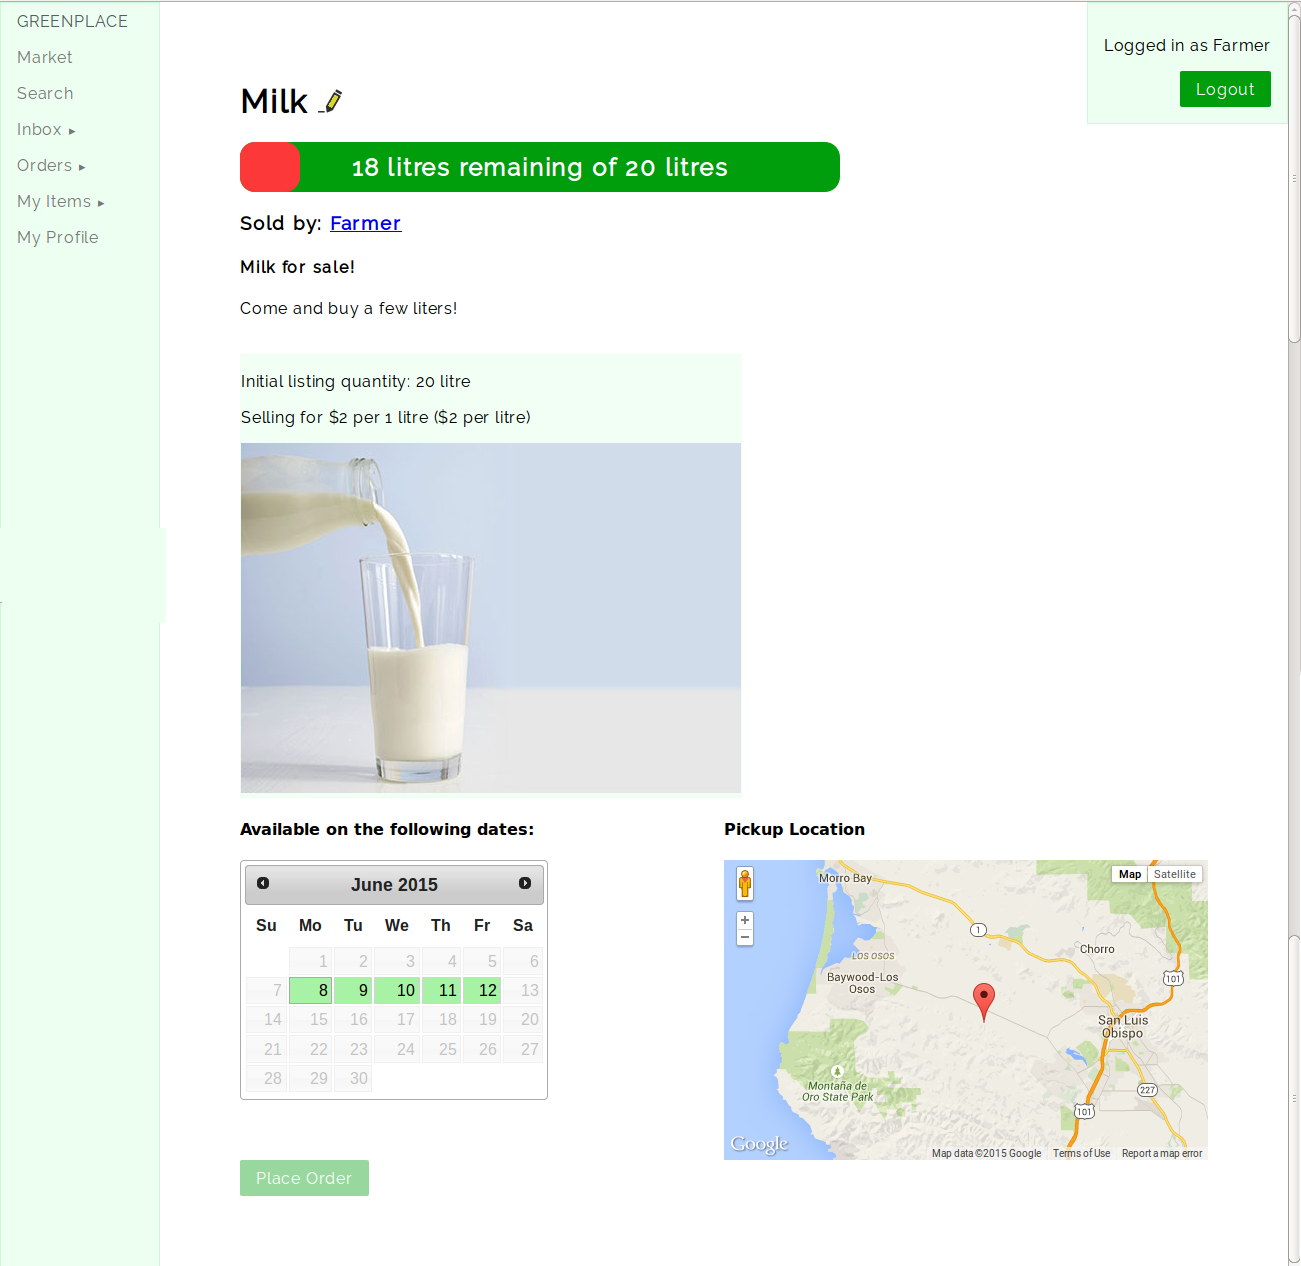
\includegraphics[width=\textwidth]{images/item.png}
\end{figure}

\begin{figure}[H]
  \caption{Edit Item}
  Template with prefilled information to streamline making changes to an existing item.\\
  \label{fig:itemedit}
  \centering
    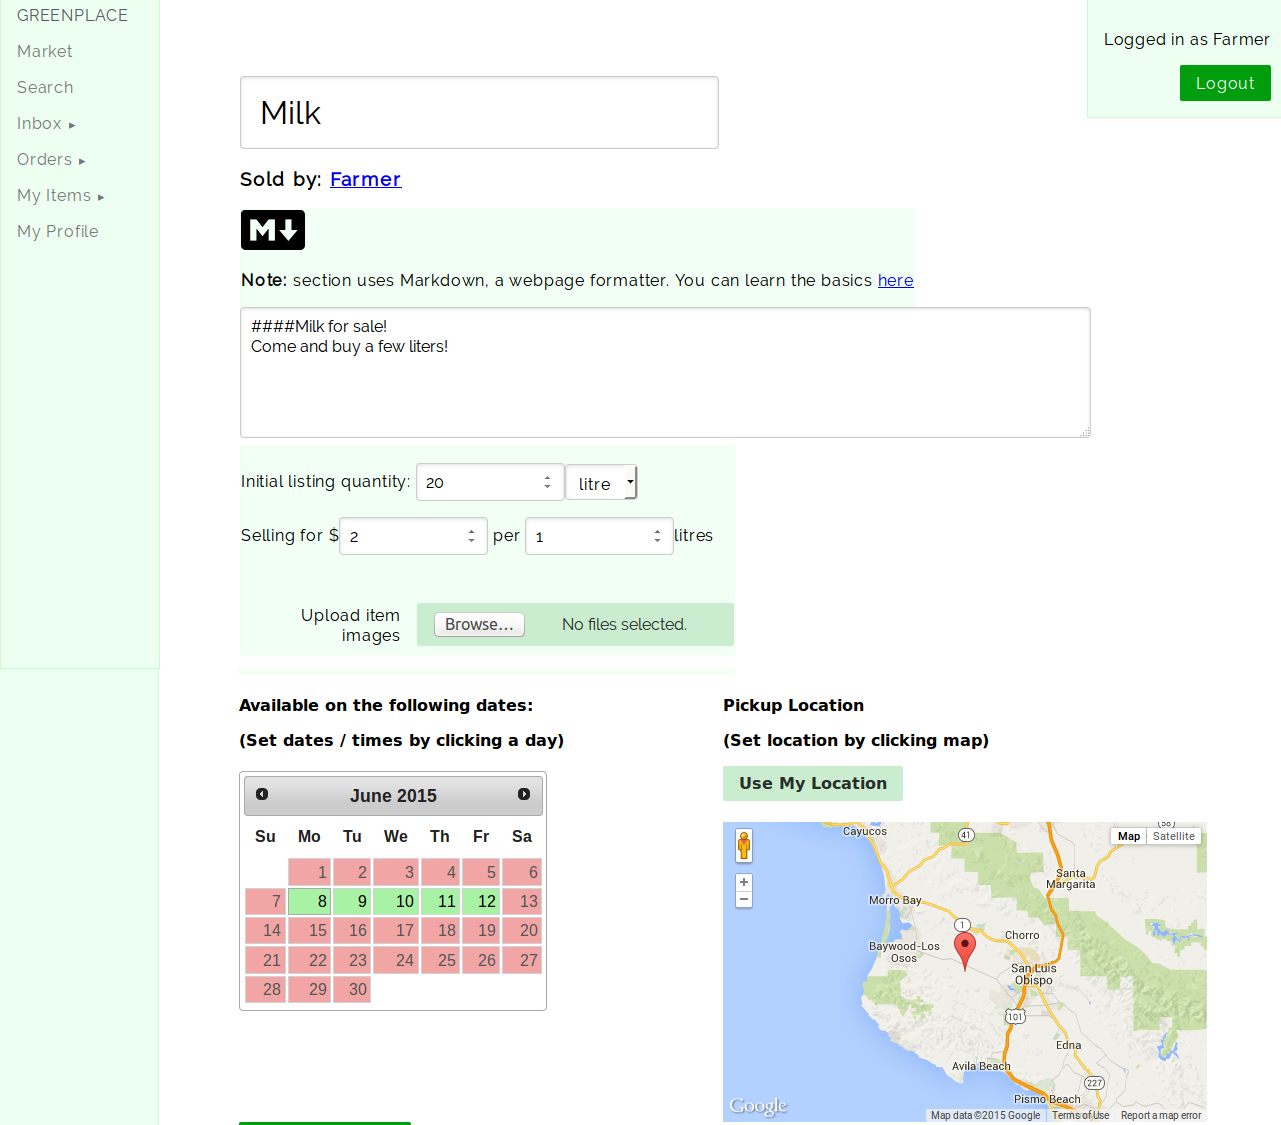
\includegraphics[width=\textwidth]{images/itemedit.png}
\end{figure}

\begin{figure}[H]
  \caption{My Items}
  Table displaying all products for sale by the authenticated user available for purchase.\\
  \label{fig:myitems}
  \centering
    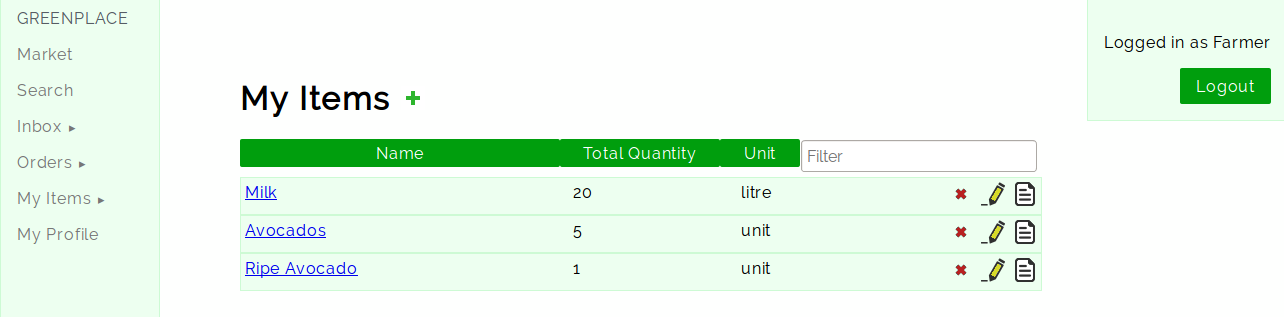
\includegraphics[width=\textwidth]{images/myitems.png}
\end{figure}

\begin{figure}[H]
  \caption{My Orders}
  Orders that have been placed by the logged in user on products interested in purchasing.\\
  \label{fig:myorders}
  \centering
    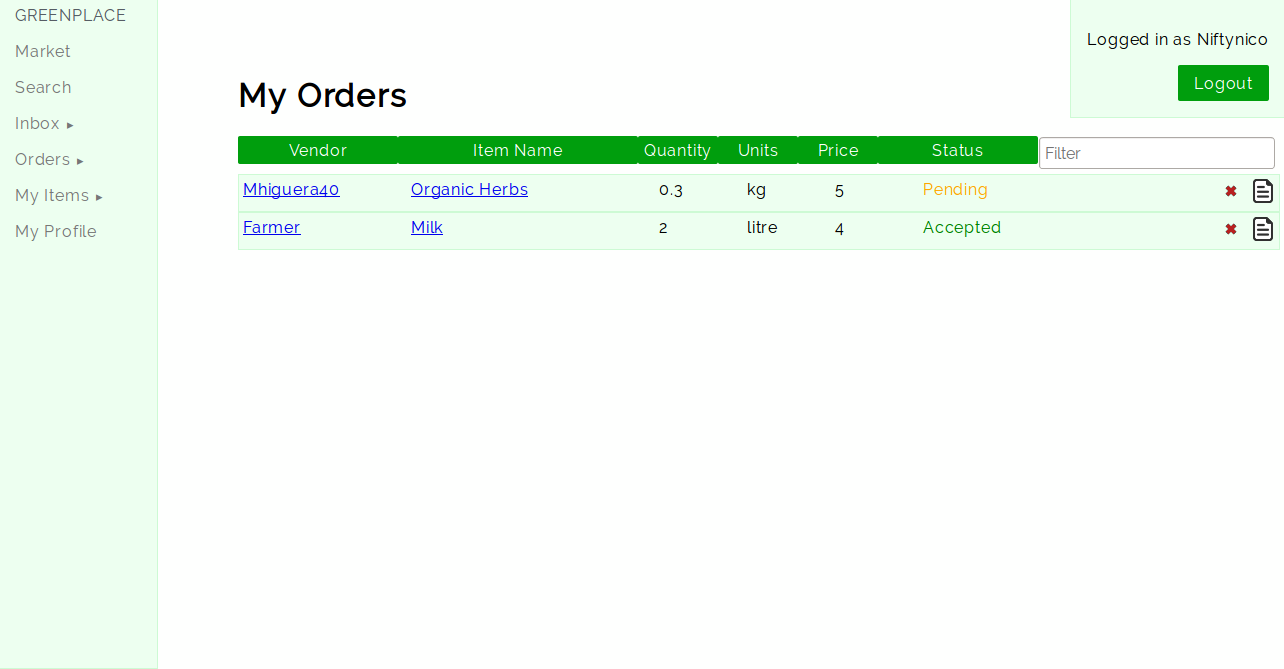
\includegraphics[width=\textwidth]{images/myorders.png}
\end{figure}

\begin{figure}[H]
  \caption{View Order}
  Detailed information regarding a potential product purchase. In this case, the order was declined by the vendor.\\
  \label{fig:orderview}
  \centering
    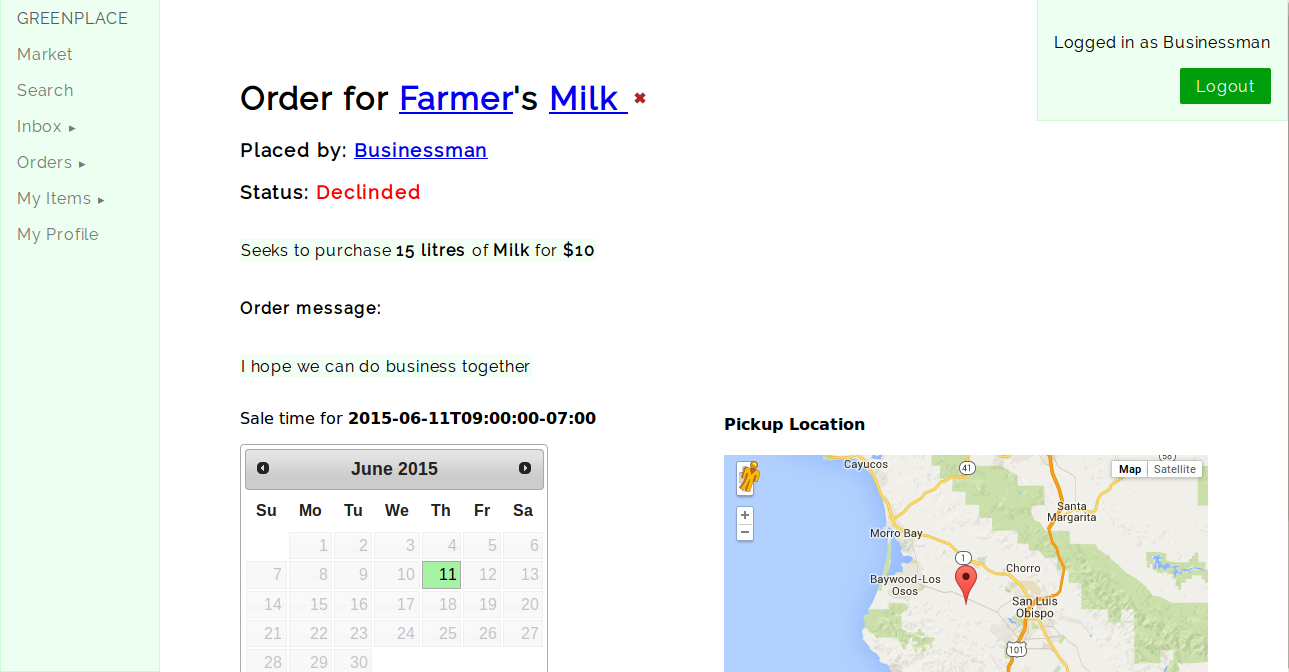
\includegraphics[width=\textwidth]{images/orderview.png}
\end{figure}

\begin{figure}[H]
  \caption{Customer Orders}
  Orders that have been placed on one of the logged in user's products.\\
  \label{fig:customerorders}
  \centering
    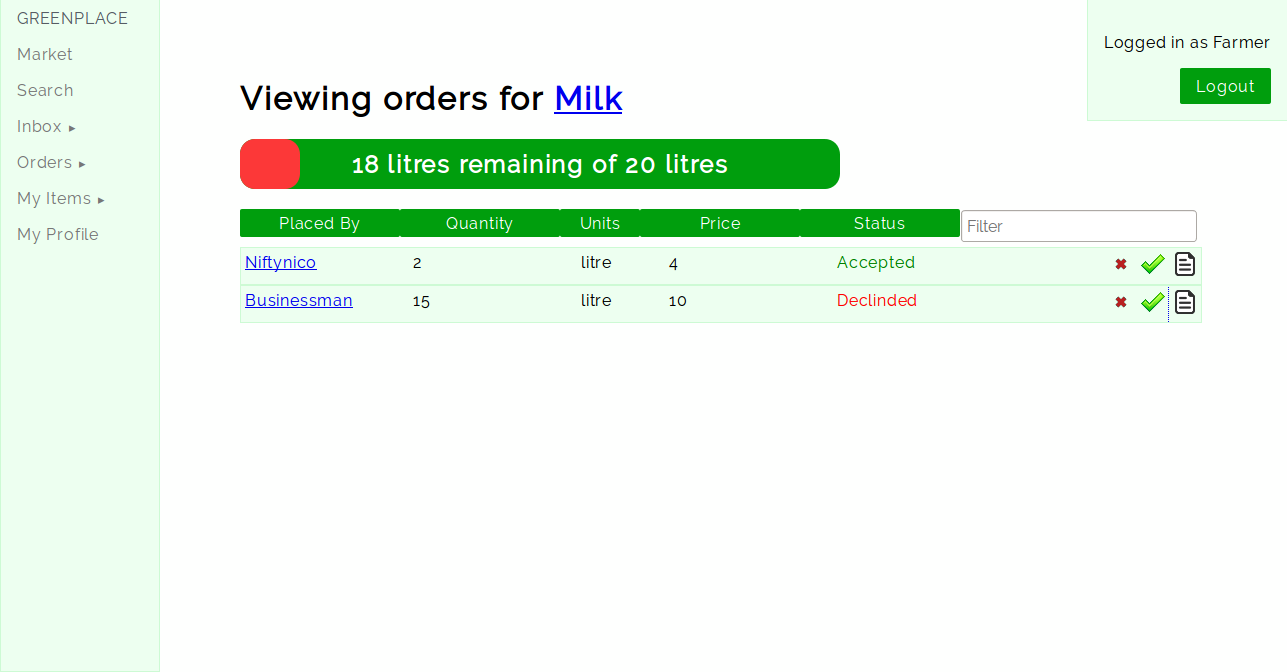
\includegraphics[width=\textwidth]{images/customerorders.png}
\end{figure}

\begin{figure}[H]
  \caption{Profile}
  A customizeable profile displaying relevant merchant information about the user. Changes can be made by the authenticated user by clicking the pencil.\\
  \label{fig:profile}
  \centering
    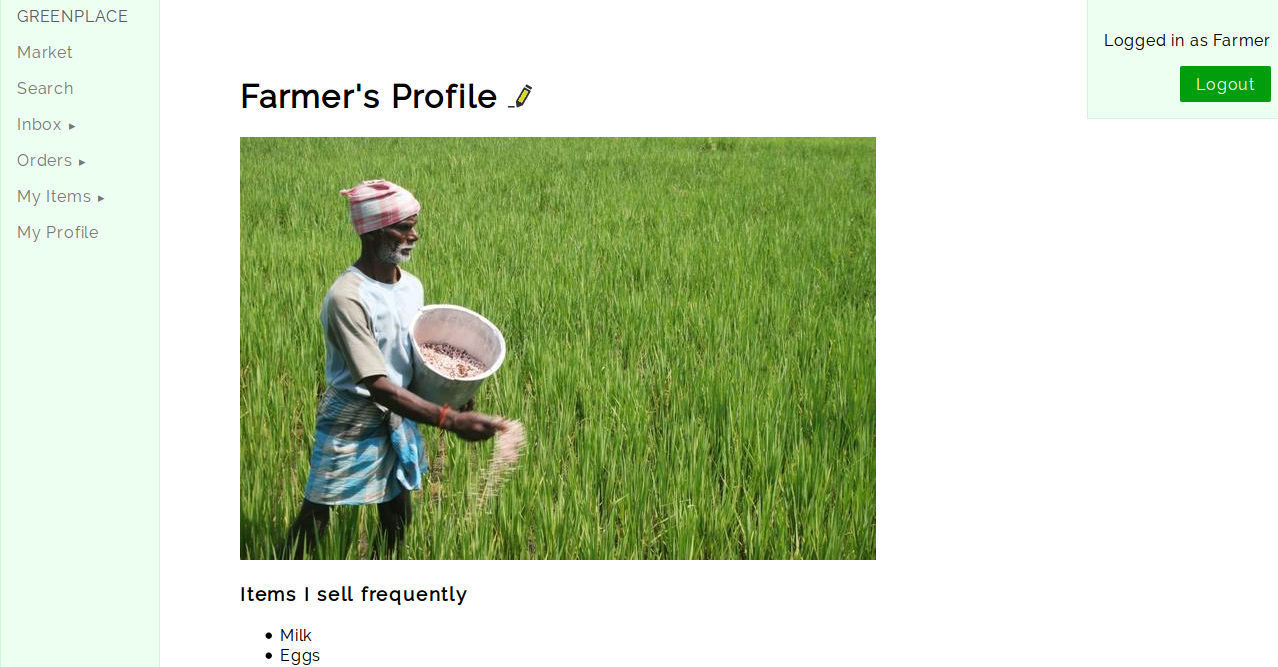
\includegraphics[width=\textwidth]{images/profile.png}
\end{figure}

\begin{figure}[H]
  \caption{Messages Received}
  Displays messages sent from other users to that which is currently authenticated.\\
  \label{fig:receivedmessages}
  \centering
    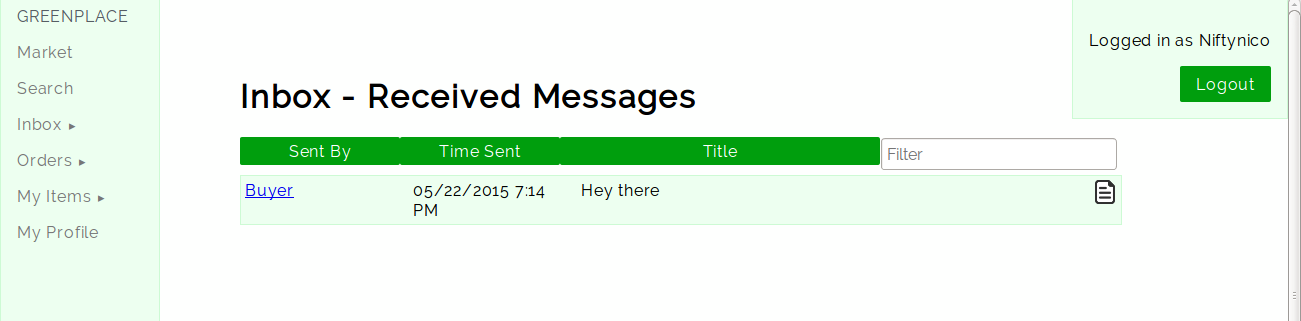
\includegraphics[width=\textwidth]{images/inbox-received.png}
\end{figure}

\begin{figure}[H]
  \caption{View Message}
  A message sent to the currently authenticated user.\\
  \label{fig:message}
  \centering
    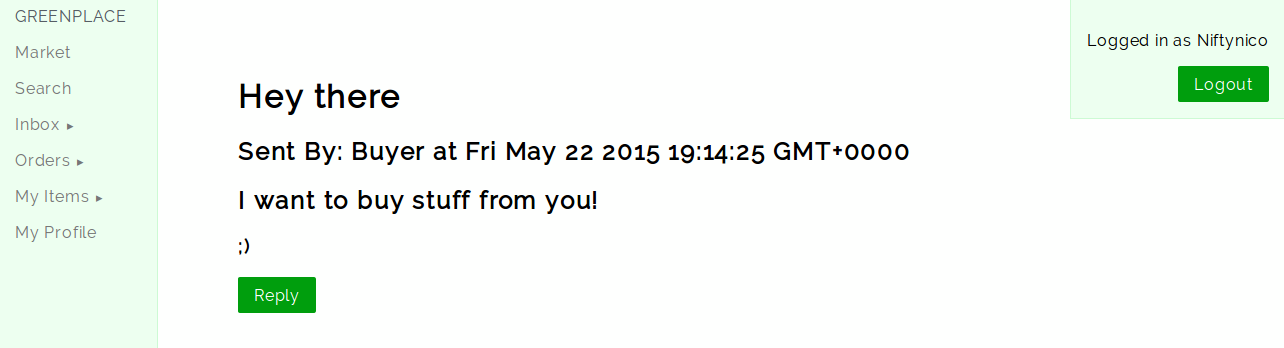
\includegraphics[width=\textwidth]{images/message.png}
\end{figure}

\begin{figure}[H]
  \caption{Compose Message}
  Compose a message to be sent to another user using markdown formatted text.\\
  \label{fig:composemessage}
  \centering
    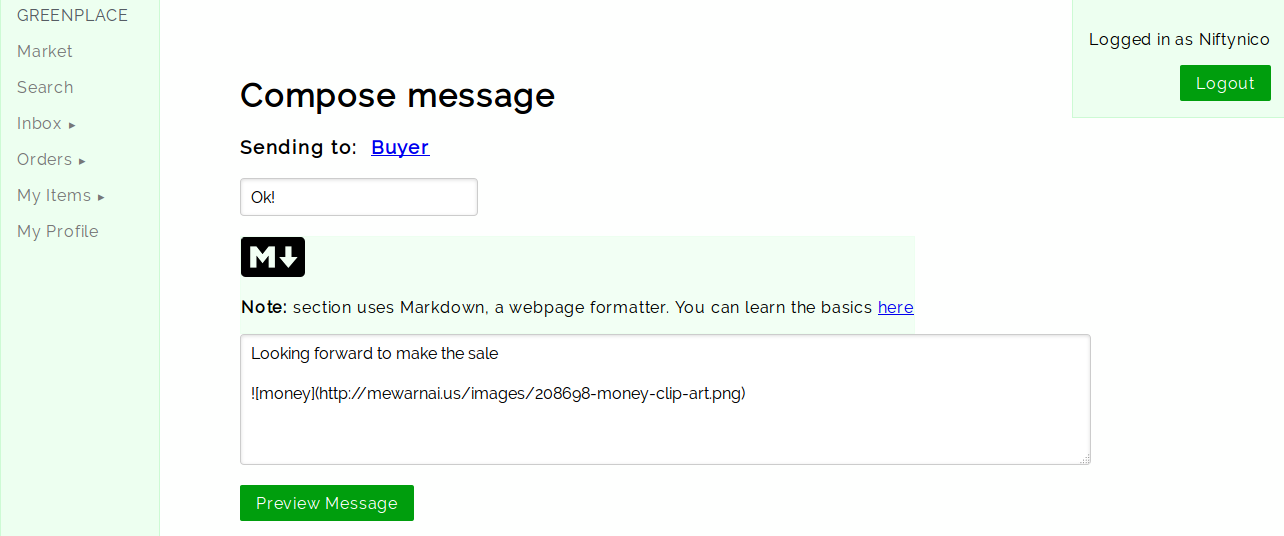
\includegraphics[width=\textwidth]{images/composemessage.png}
\end{figure}

\begin{figure}[H]
  \caption{Preview Message}
  Preview message to verify properly formatted text before sending.\\
  \label{fig:previewmessage}
  \centering
    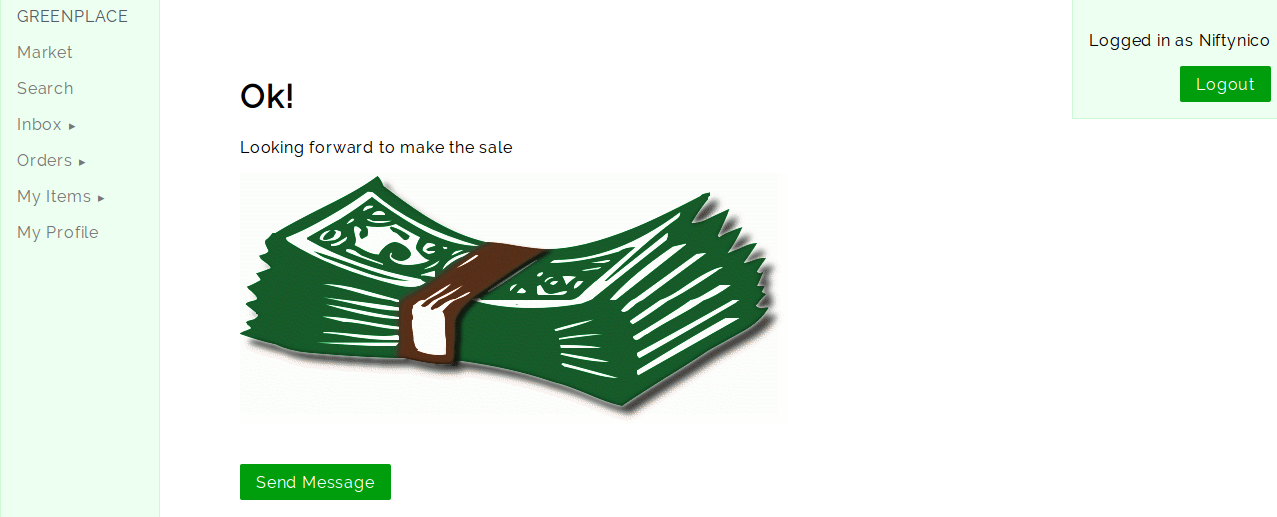
\includegraphics[width=\textwidth]{images/previewmessage.png}
\end{figure}

\subsection{Special Thanks}

\begin{itemize}
  \item Adam Currie for creating the query that searches the database for matching products given keywords, location, availability, and minimum or maximum quantity
  \item Justin Fujikawa for adding functionality to allow users to edit their description using markdown text.
  \item Dr. Clark Savage Turner and Dr. Philip Nico for guidance during the project.
\end{itemize}

\end{document}
